
\documentclass[letterpaper,landscape,english,9pt]{report}
\usepackage[landscape,margin=0.5cm]{geometry}

\usepackage{fixltx2e} % LaTeX patches, \textsubscript
\usepackage{cmap} % fix search and cut-and-paste in PDF
\usepackage[T1]{fontenc}
\usepackage[utf8]{inputenc}
\usepackage{ifthen}
\usepackage{babel}
\usepackage{color}
\usepackage{float} % float configuration
\floatplacement{figure}{H} % place figures here definitely


\usepackage{multicol}
%\setlength{\columnseprule}{1pt} % for visible divider
\setlength{\columnsep}{1cm}

\usepackage{graphicx}
\graphicspath{
 {../pics/}
}

%%% Custom LaTeX preamble
% PDF Standard Fonts
\usepackage{mathptmx} % Times
\usepackage[scaled=.90]{helvet}
\usepackage{courier}

\usepackage{flowfram}
%\usepackage{booktabs}           % for rules in tables
\usepackage{tabularx}           % for column-width tables
\usepackage[table]{xcolor}      % color control

%\usepackage[colorlinks]{hyperref}

\usepackage{enumitem}           % useful for control of listings
\usepackage[compact,raggedright]{titlesec}
\usepackage{comment}

\newcommand{\epigraph}[3]{\textit{#1}\linebreak \vspace{-1.5em} \begin{flushright}\hspace{5em}\ --\ #2\linebreak\small{#3} \end{flushright}}

\pagestyle{empty}
\parindent=0pt

% Attempts to change bg color of *section headings
%\definecolor{secbgcol}{rgb}{0.9, 0.85, 0.85}
%\titleformat{\section}
%{\color{red}\normalfont\Large\bfseries}{\ndsection}{1em}{}
%\titleformat{\subsection}
%{\color{red}\normalfont\large\bfseries}{\begin{flushright}\hfill\thesubsection
%  \end{flushright}}{1em}{}
%
%\usepackage{pstricks}

% To create tables within multicols
\makeatletter
\newenvironment{ndtable}
  {\def\@captype{table}}
  {}


\newcommand{\ndheading}[3]{%
\vspace{0.5em}
\begin{ndtable}%
\rowcolors[\hline]{1}{#2}{} \arrayrulecolor{#3}
\begin{tabularx}{\columnwidth}{>{\centering\arraybackslash}X}\vspace{-.5em}\normalfont\large\bfseries
  #1\vspace{0.05em}\\\end{tabularx}
\end{ndtable}
\vspace{-.5em}
}

\definecolor{secfgcol}{RGB}{102, 153, 0}
\definecolor{secbgcol}{RGB}{216, 255, 137}
\definecolor{projfgcol}{RGB}{6,   83, 215}
\definecolor{projbgcol}{RGB}{255, 255, 205}

%\definecolor{secfgcol}{RGB}{6, 83, 215}
%\definecolor{secbgcol}{RGB}{241, 248, 255}
%\definecolor{projfgcol}{RGB}{6,   83, 215}
%\definecolor{projbgcol}{RGB}{241, 248, 255}

\newcommand{\ndsection}[1]{\ndheading{#1}{secbgcol}{secfgcol}}
\newcommand{\ndsubsection}[1]{\ndheading{#1}{secbgcol}{secfgcol}}

%\newcommand{\ndproject}[2]{\ndheading{\noindent#1\newline{\small\url{#2}}}{secbgcol}{secfgcol}}

\newcolumntype{V}{>{\arraybackslash} m{.2\linewidth} }
\newcolumntype{C}{>{\arraybackslash} m{.72\linewidth} }
\newcommand{\ndproject}[6]{%
\vspace{0.5em}
\begin{ndtable}%
\rowcolors[]{1}{projbgcol}{} \arrayrulecolor{projbgcol}
\begin{tabularx}{\columnwidth}{CV}\vspace{-.5em}\normalfont\large\bfseries
 #1 \newline {\small\url{#2}} &
 \vspace{#5}\hspace{#6}\includegraphics[width=#4\columnwidth]{../pics/#3}\vspace{-0.5em}\end{tabularx}
\end{ndtable}
\vspace{-.5em}
}

\newcommand{\ndcite}[1]{{\small #1}}
%%% User specified packages and stylesheets

%%% Fallback definitions for Docutils-specific commands

% admonition (specially marked topic)
\providecommand{\DUadmonition}[2][class-arg]{%
  % try \DUadmonition#1{#2}:
  \ifcsname DUadmonition#1\endcsname%
    \csname DUadmonition#1\endcsname{#2}%
  \else
    \begin{center}
      \fbox{\parbox{0.9\textwidth}{#2}}
    \end{center}
  \fi
}

% title for topics, admonitions and sidebar
\providecommand*{\DUtitle}[2][class-arg]{%
  % call \DUtitle#1{#2} if it exists:
  \ifcsname DUtitle#1\endcsname%
    \csname DUtitle#1\endcsname{#2}%
  \else
    \smallskip\noindent\textbf{#2}\smallskip%
  \fi
}

% hyperlinks:
\ifthenelse{\isundefined{\hypersetup}}{
  \usepackage[unicode,colorlinks=true,linkcolor=blue,urlcolor=blue]{hyperref}
  \urlstyle{same} % normal text font (alternatives: tt, rm, sf)
}{}

%%% Local Variables:
%%% mode: latex
%%% TeX-master: t
%%% TeX-PDF-mode: t
%%% End:


\hypersetup{
  pdftitle={Python in Electrophysiology},
}

%%% Body
\begin{document}

\begin{multicols}{3}    % 3 columns

% Document title
%\section*{
\begin{center}\Large \textbf{Python in Electrophysiology}\end{center}
%}
%\label{python-in-neuroimaging}

\begin{center}
\noindent
%% yoh: what logo?  worse comes to worse we could reuse snakebrain in
%%      different colorscheme ;)
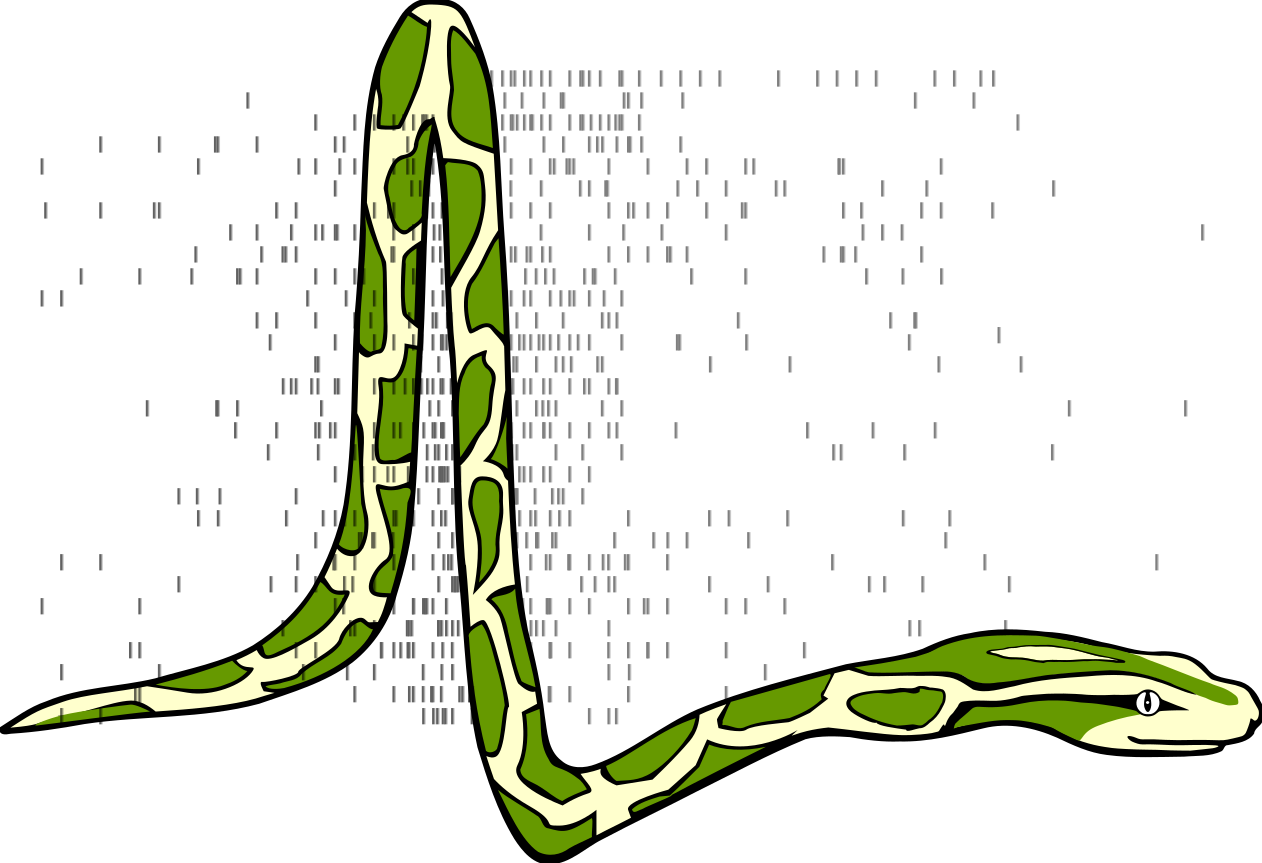
\includegraphics[width=0.7\columnwidth]{python_action_potential}
%\includegraphics[width=0.5\columnwidth]{openlogo-vsop}

Find the community @ \url{http://neuralensemble.org}

%% yoh: or what should be(come) the canonical location?
%%      or should we (you) come up with one?

% \hrule
\end{center}
\vspace{0em}


%___________________________________________________________________________
%% yoh: what sections do you foresee?  Below see my blunt dump of ideas
%%      or may be there should be no sections at all?

\ndsection{Data I/O}

%___________________________________________________________________________

% Your logo placed under ../pics called as <project>_logo.svg
% .svg is preferable, otherwise some other vector (.pdf) or even
% raster (.png) would suffice
\ndproject{XXX}{http://example.org}{opensesame_logo.pdf}{.2}{-0.25em}{0em}

%\begin{figure}
%
\includegraphics[width=0.3\columnwidth]{../pics/psychopy_logo.pdf}
%\end{figure}

Brief description.
\begin{itemize}[nolistsep,topsep=0em,leftmargin=1pc]
\item The most interesting
\item and
\item methodology oriented
\item features
\item ideally with limited selection of citations
\end{itemize}
% Your favorite screenshot placed under ../pics/
% named as <project>_screenshot.png (optional numbers in suffixes if
% you have multiple to choose from)
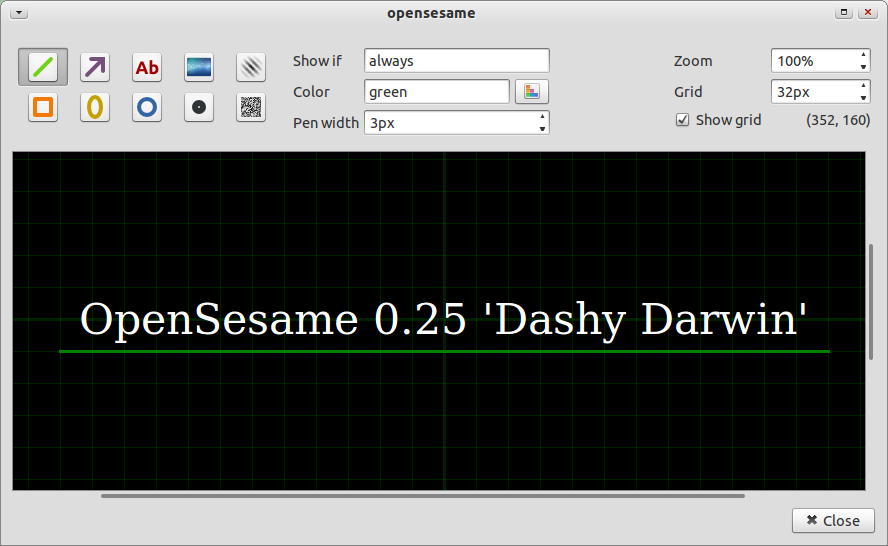
\includegraphics[width=\columnwidth]{opensesame_screenshot1.png}
% Selected set of citations, Here is an example:
\ndcite{D. Geffroy, D. Rivière, I. Denghien, N. Souedet,
  S. Laguitton, and Y. Cointepas. BrainVISA: a complete software
  platform for neuroimaging.  In Python in Neuroscience workshop,
  Paris, Aug. 2011.}


\ndproject{Neuroshare Tools}{http://g-node.org/neuroshare-tools}{neurosharelogo_square.png}{.2}{-0.25em}{0em}

Neuroshare is a standardized API for accessing neurophysiology
data stored in vendor-specific binary formats in a vendor-neutral
way. The G-Node Neuroshare Tools provide libraries and utilities
built on Neuroshare and Python to work with Neuroshare compatible
files on various platforms.

\begin{itemize}[nolistsep,topsep=0em,leftmargin=1pc]
\item High-level Python library to access Neuroshare compatible data-files
\item Automatically detects file types and loads the corresponding vendor library
\item Support for GNU/Linux, MacOS~X, and Windows
\item Neuroshare-WineProxy enables the use of vendor libraries for Windows under GNU/Linux and MacOS~X
\item Comes with a tool to convert any data file supported by Neuroshare to the HDF5 format
\end{itemize}

%_________________________________neo_______________________________________
\ndproject{Neo}{http://packages.python.org/neo/}{neo_logo.png}{.2}{-0.25em}{0em}

Neo is a package for representing electrophysiology data in Python, together with support
for reading a wide range of neurophysiology file formats, including Spike2, NeuroExplorer,
AlphaOmega, Axon, Blackrock, Plexon, Tdt, and support for writing to a subset of these
formats plus non-proprietary formats including HDF5.

The goal of Neo is to improve interoperability between Python tools for analyzing, visualizing
and generating electrophysiology data (such as OpenElectrophy, NeuroTools, G-node,
Helmholtz, PyNN) by providing a common, shared object model. In order to be as
lightweight a dependency as possible, Neo is deliberately limited to represention of data,
with no functions for data analysis or visualization.

Neo implements a hierarchical data model well adapted to intracellular and extracellular
electrophysiology and EEG data with support for multi-electrodes (for example tetrodes).
Neo's data objects build on the quantities package, which in turn builds on NumPy by 
adding support for physical dimensions. Thus Neo objects behave just like normal NumPy arrays,
but with additional metadata, checks for dimensional consistency and automatic unit conversion.

A project with similar aims but for neuroimaging file formats is NiBabel.


%____________________OpenElectrophy______________________________________

\ndproject{OpenElectrophy}{http://packages.python.org/OpenElectrophy/}{OpenElectrophy_logo.png}{.2}{-0.25em}{0em}

OpenElectrophy is build on top of neo.

\begin{itemize}[nolistsep,topsep=0em,leftmargin=1pc]
\item A GUI on top of neo.
\item A collection of method for spike sorting and powerfull GUI.
\item A wavelet method for analysing transient oscillations in LFP.
\item A customisable database to organize datasets.
\end{itemize}

%___________________________________________________________________________

%___________________________________________________________________________
\ndsection{Metadata Management}%

\ndproject{odML libraries \& Editor}{http://www.g-node.org/odml/}{odml_logo.pdf}{.2}{-0.25em}{0em}

Use the {open metadata Markup Language} to annotate data with information about the stimulus, data acquisition, and experimental conditions.

\begin{itemize}[nolistsep,topsep=0em,leftmargin=1pc]
\item Developer friendly libraries for Python and Java
\item Fully functional graphical editor for Linux, Windows, and MacOS~X
\item Support for the latest odML specification
\end{itemize}

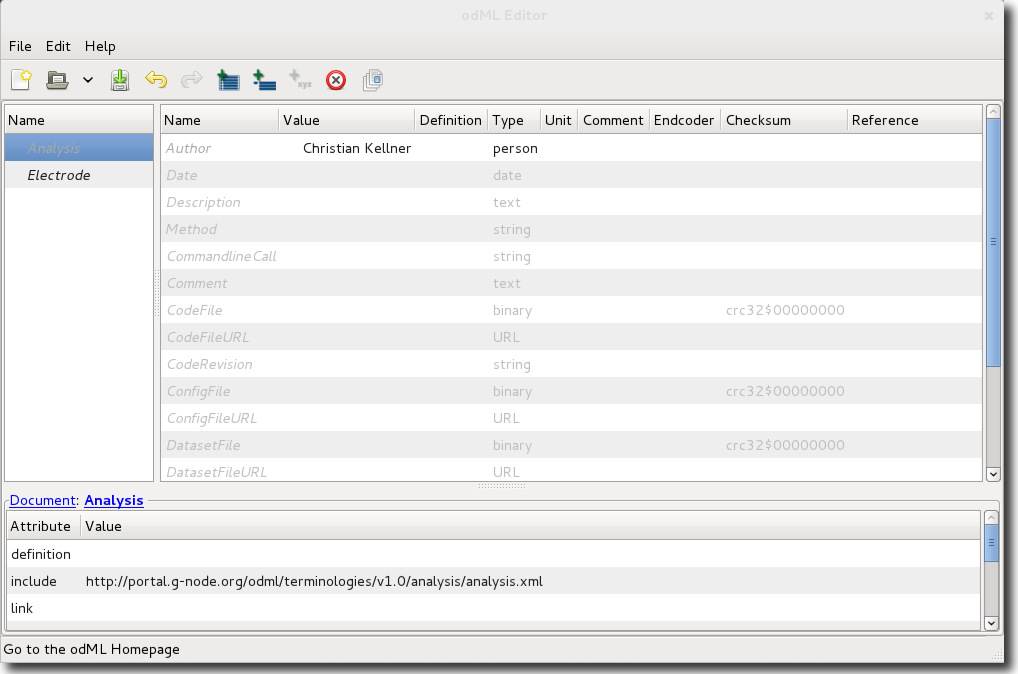
\includegraphics[width=\columnwidth]{odml_editor_screenshot.png}

\ndcite{Grewe J, Wachtler T, Benda J (2011) A bottom-up approach to data annotation in neurophysiology. Front. Neuroinform. 5:16. doi:~10.3389/fninf.2011.00016\\}
\ndsection{Data Archiving}
\ndsection{Experimentation Control}
\ndsection{Analysis}%

%________________________Stimfit____________________________________________

% Your logo placed under ../pics called as <project>_logo.svg
% .svg is preferable, otherwise some other vector (.pdf) or even
% raster (.png) would suffice
\ndproject{Stimfit}{http://www.stimfit.org}{stimfit_logo.png}{.2}{-0.25em}{0em}

%\begin{figure}
%
\includegraphics[width=0.3\columnwidth]{../pics/psychopy_logo.pdf}
%\end{figure}

Visualise and quantify electrophysiological data.
\begin{itemize}[nolistsep,topsep=0em,leftmargin=1pc]
\item With a focus on patch-clamp recordings
\item Supports most standard patch-clamp file types
\item Embedded Python shell
\item Measure action potential, EPSC and EPSP kinetics
\item Extract spontaneous and evoked events
\item Successfully used in many publications for >\,5 years
\end{itemize}
% Your favorite screenshot placed under ../pics/
% named as <project>_screenshot.png (optional numbers in suffixes if
% you have multiple to choose from)
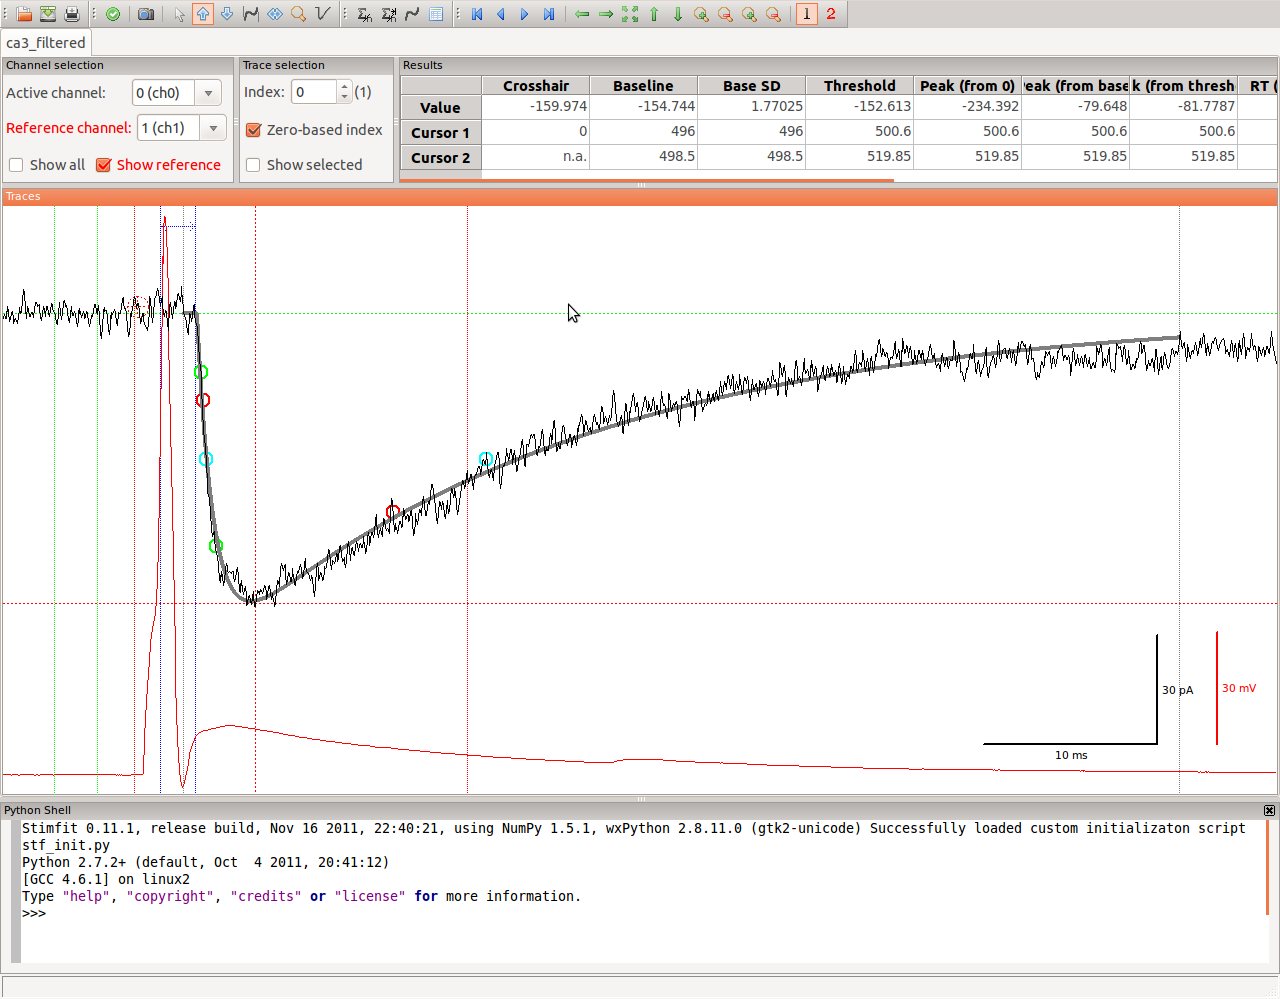
\includegraphics[width=\columnwidth]{stimfit_screenshot.png}
% Selected set of citations, Here is an example:
% Working on a manuscript right now ;-)

%___________________________________________________________________________

\ndsection{Closed-loop Frameworks}%

\end{multicols}
\end{document}

%%% Local Variables:
%%% mode: latex
%%% TeX-master: t
%%% TeX-PDF-mode: t
%%% whizzy-viewers: (("-pdf" "okular") ("-dvi" "xdvi") ("-ps" "gv"))
%%% End:
